% !TEX options=--shell-escape
\documentclass [12pt]{article} 
\usepackage {amsmath}
\usepackage {amsthm}
\usepackage {amssymb}
\usepackage {graphicx} 
\usepackage {float}
\usepackage {multirow}
\usepackage {xcolor}
\usepackage {algorithmic}
\usepackage [ruled,vlined,commentsnumbered,titlenotnumbered]{algorithm2e} \usepackage {array} 
\usepackage {booktabs} 
\usepackage {url} 
\usepackage {parskip} 
\usepackage [margin=1in]{geometry} 
\usepackage [T1]{fontenc} 
\usepackage {cmbright} 
\usepackage [many]{tcolorbox} 
\usepackage [colorlinks = true,
            linkcolor = blue,
            urlcolor  = blue,
            citecolor = blue,
            anchorcolor = blue]{hyperref} 
\usepackage {enumitem} 
\usepackage {xparse} 
\usepackage {verbatim}
\usepackage{listings}
\usepackage{xcolor}
\usepackage{csquotes}
\usepackage[cache=false]{minted}
\usepackage{mdframed}
\usepackage{tikz}
\usetikzlibrary{shapes.symbols}
\newtheorem{theorem}{Theorem}

\DeclareTColorBox {Solution}{}{breakable, title={Solution}}
\DeclareTColorBox {Solution*}{}{breakable, title={Solution (provided)}}
\DeclareTColorBox {Instruction}{}{boxrule=0pt, boxsep=0pt, left=0.5em, right=0.5em, top=0.5em, bottom=0.5em, arc=0pt, toprule=1pt, bottomrule=1pt}
\DeclareDocumentCommand {\Expecting }{+m}{\textbf {[We are expecting:} #1\textbf {]}}
\DeclareDocumentCommand {\Points }{m}{\textbf {(#1 pt.)}} 
\newcommand {\hint }[1]{\noindent {[\textbf {HINT:} \em #1 \em ]}} \newcommand {\pts }[1]{\textbf {(#1 pt.)}} 

\begin{document} 

{\LARGE \textbf {COMP 285 (NC A\&T, Spr `22)}\hfill \textbf {Weekly Quiz 2} } 

\section{} Consider the following graph, where the weights (the numbers on the edges) are meant to represent the cost of walking along an edge.
Suppose you do BFS starting at the node A. What does BFS find as the shortest path from A to C?
\begin{figure}[H]
    \centering
    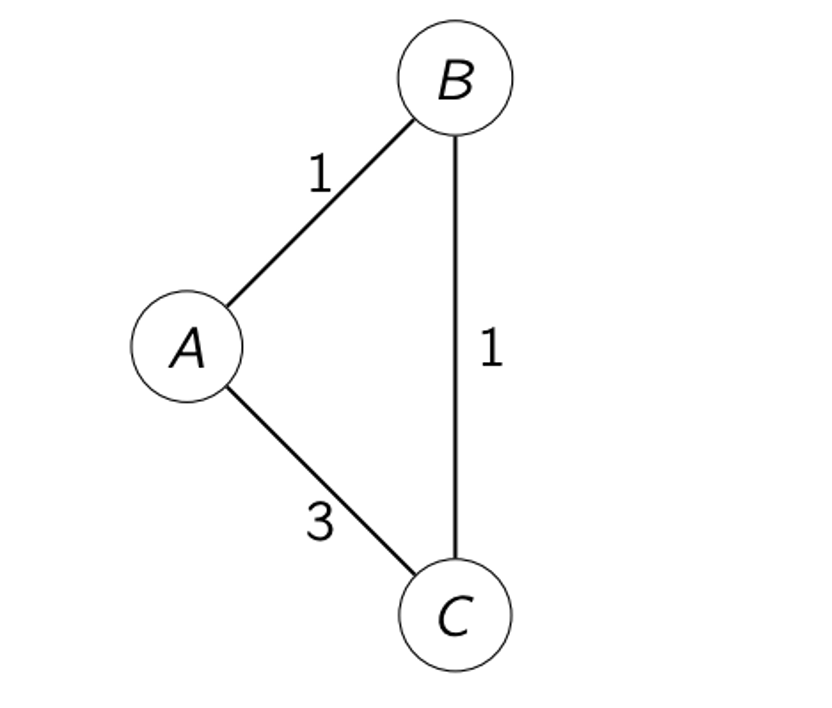
\includegraphics[scale=0.5]{7.png} 
    \label{fig:my_label}
\end{figure}

\begin{Solution}
The path $A \to C$
\paragraph{}
Note that the edges represent the cost but BFS ignores this.
\end{Solution}


\section{} If you take the weights into account, what is the shortest path from A to C? (By ``take the weights into account'' we mean add up the weights along each path the get the length of a path. So, with the weights, the cost of the path A → C → B would be 3 + 1 = 4.)
\begin{figure}[H]
    \centering
    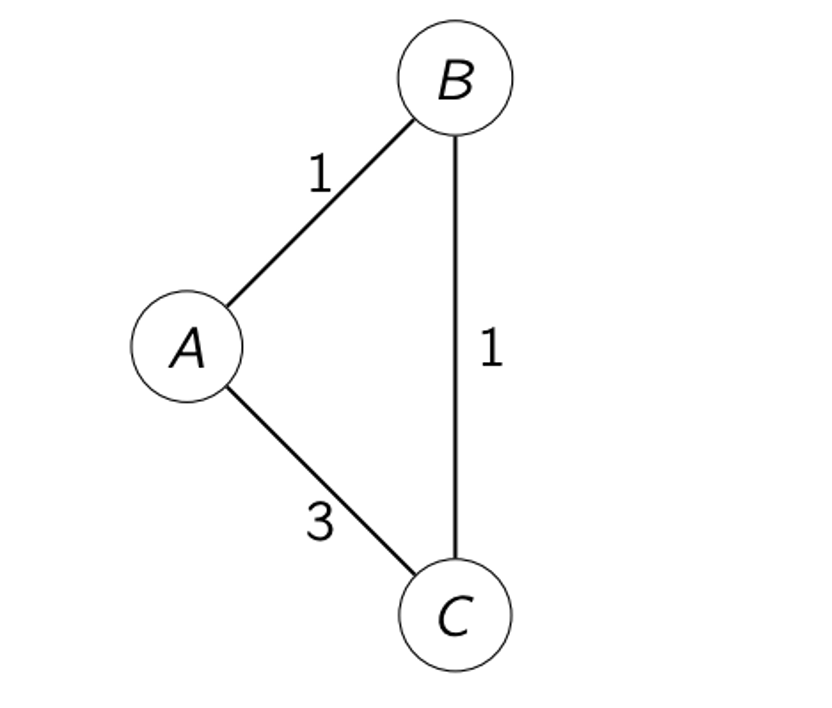
\includegraphics[scale=0.5]{7.png} 
    \label{fig:my_label}
\end{figure}

\begin{Solution}
The path $A \to B \to C$.
\end{Solution}


\section{} Suppose that we want to find the shortest path between two nodes in the following graph. Which algorithm can we use?
\begin{figure}[H]
    \centering
    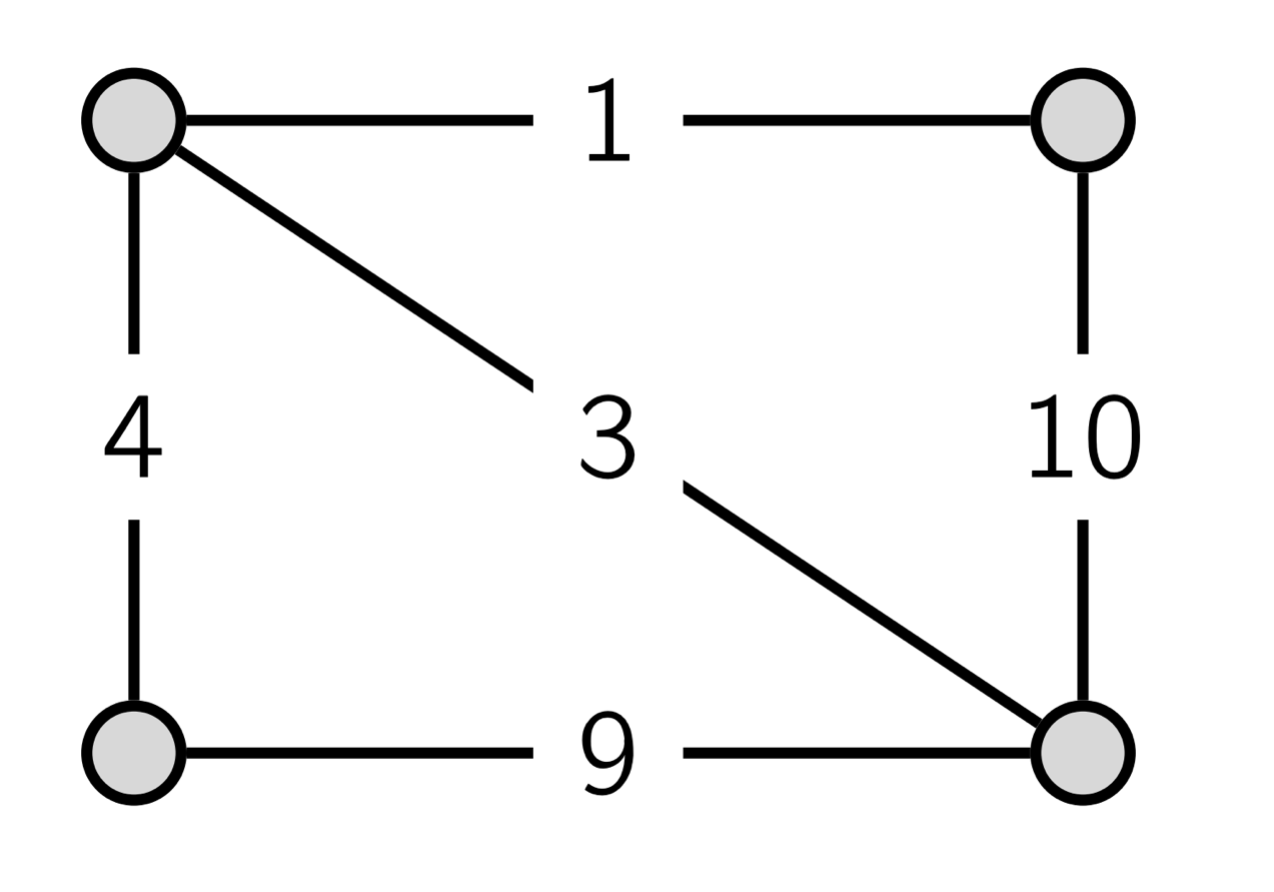
\includegraphics[scale=0.5]{8.png} 
    \label{fig:my_label}
\end{figure}

\begin{Solution}
Dijkstra's Algorithm because the graph is weighted but has no negative edge weights.
\end{Solution}


\section{} Select all the scenarios where we can use Dijkstra's Algorithm to find the shortest paths.

\begin{Solution}
\begin{itemize}
    \item An undirected graph with positive edge weights
    \item A directed graph with positive edge weights
\end{itemize}
\end{Solution}


\section{} Dijkstra Forensics
\paragraph{}
Suppose we run Dijkstra on some graph with nodes A, B, C, D, E, F that has nonnegative ($\geq 0$) edge weights, starting from the node A. In the middle of the algorithm our computer crashes. We look through the memory dump, and see that the state of $d$ looked as follows when the crash happened: 
\begin{align*}
d[A] = 0 \\
d[B] = 5 \\ 
d[C] = 4 \\ 
d[D] = 15 \\
d[E] = 2 \\
d[F] = 20 
\end{align*}.
Additionally from the memory dump we see that the current node when the crash happened was node C.
\paragraph{}
What is the minimum possible length of the shortest path from node A to node B?

\begin{Solution}
We know that $B$ hasn't been started yet because we're on C and B's estimate is larger. As such, the minimum possible length is because C is the smallest not-yet-finished node and it has path of length 4.
\end{Solution}


\section{} What is the maximum possible length of the shortest path from node A to node B?

\begin{Solution}
5 because this is d[B] which is an upper-bound (overestimate) on the shortest path from A to node B.
\end{Solution}


\section{} What is the minimum possible length of the shortest path from node A to node E?

\begin{Solution}
2 because it's the value stored in d[E] and E is "done" since we're processing C which has shortest path of 4.
\end{Solution}


\section{} What is the maximum possible length of the shortest path from node A to node E?

\begin{Solution}
2 because this is d[E] which is an upper-bound (overestimate) on the shortest path from A to node B. In fact, node $E$ has been completed already, so its estimate is its shortest path.
\end{Solution}


\section{} If we run the Dijkstra algorithm on the graph of U.S. streets/roads/highways/etc., starting from the Greensboro Science Center, which of the following locations will become the current node first?

\begin{Solution}
Bandito Burrito in Greensboro
\paragraph{}
Compared with Times Square in New York, and the Hollywood Sign, this is closer to the Greensboro Science Center.
\end{Solution}

\end{document} 